\documentclass{standalone}
\usepackage{tikz}


\begin{document}
    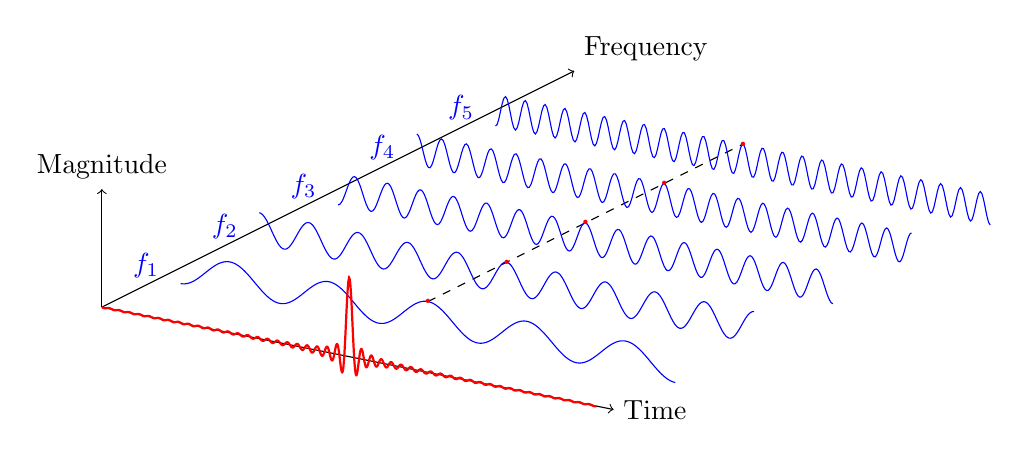
\begin{tikzpicture}[x={(1cm,0.5cm)},z={(0cm,1cm)},y={(1cm,-0.2cm)}]

        %repere
        \draw[->] (0,-pi,0) --++ (6,0,0) node[above right] {Frequency};
        \draw[->] (0,-pi,0) --++ (0,6.5,0) node[right] {Time};
        \draw[->] (0,-pi,0) --++ (0,0,1.5) node[above] {Magnitude};

        \draw [dashed] (1,0,0.2) --++ (4,0,0);          
        \foreach \y in {1,2,...,5}{
            %sinusoides
            \draw[blue] plot[domain = -pi:+pi, samples = 300] 
            (\y,\x,{0.2*cos(10*\y/2*(\x) r)});
            \draw[blue] (\y,-pi-0.15,0) node [left]{$f_{\y}$};
            \draw[red] (\y,0,{0.2*cos(10*\y/2*(0) r)}) node {\textbf{.}};
        }

        %sinc
        \draw[red, thick] plot[domain = -pi:+pi, samples = 2000] 
        (0,\x,{0.02*sin(50*(\x) r)/(\x))});

    \end{tikzpicture}
\end{document}
